\documentclass[11pt]{article}
\usepackage[margin=1in]{geometry}
\usepackage{graphicx}
\usepackage{booktabs}
\usepackage{hyperref}
\usepackage{float}
\usepackage{caption}
\usepackage{subcaption}
\usepackage{amsmath}
\usepackage{enumitem}

\title{\textbf{Project 5: Recognition Using Deep Networks}}
\author{Divya Vinaybhai Patel}
\date{April 2026}

\begin{document}
\maketitle

% ============================================================
\section{Project Overview}
% ============================================================

This project explores building, training, analyzing, and modifying deep neural networks for image recognition tasks. Using the MNIST handwritten digit dataset, I implemented a Convolutional Neural Network (CNN) that achieves over 97\% test accuracy after five epochs of training. I then examined the trained network's internal representations by visualizing convolutional filters and their effects on input images. To demonstrate transfer learning, I adapted the pre-trained MNIST network to classify Greek letters (alpha, beta, gamma) by freezing learned weights and retraining only the final classification layer. I also re-implemented the recognition pipeline using a Vision Transformer (ViT) architecture, replacing convolutions with patch embeddings and self-attention. Finally, I conducted a systematic experiment on the Fashion MNIST dataset, evaluating how transformer depth, number of attention heads, and dropout rate affect classification performance using an automated round-robin search strategy.

\newpage
% ============================================================
\section{Task 1: Build and Train a Digit Recognition Network}
% ============================================================

\subsection{A -- MNIST Digit Data Set}

The MNIST dataset consists of 60,000 training and 10,000 testing 28$\times$28 grayscale images of handwritten digits (0--9). The digits appear as white strokes on a black background. Figure~\ref{fig:first_six} shows the first six examples from the test set.

\begin{figure}[H]
    \centering
    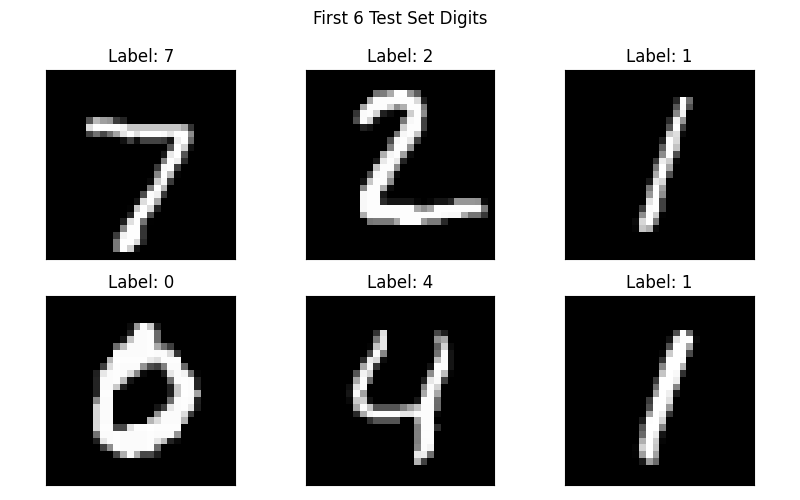
\includegraphics[width=0.75\textwidth]{plot_first_six.png}
    \caption{First six example digits from the MNIST test set. Labels shown above each image.}
    \label{fig:first_six}
\end{figure}

\subsection{B -- CNN Network Architecture}

The CNN architecture follows the specification with two convolutional layers, dropout regularization, max pooling, and two fully connected layers. Table~\ref{tab:cnn_arch} summarizes the layer structure.

\begin{table}[H]
\centering
\caption{CNN Network Architecture}
\label{tab:cnn_arch}
\begin{tabular}{@{}llll@{}}
\toprule
\textbf{Layer} & \textbf{Type} & \textbf{Details} & \textbf{Output Shape} \\
\midrule
1 & Conv2d + MaxPool2d + ReLU & 10 filters, 5$\times$5, pool 2$\times$2 & 10$\times$12$\times$12 \\
2 & Conv2d + Dropout + MaxPool2d + ReLU & 20 filters, 5$\times$5, drop 0.5, pool 2$\times$2 & 20$\times$4$\times$4 \\
3 & Flatten + Linear + ReLU & 320 $\rightarrow$ 50 nodes & 50 \\
4 & Linear + LogSoftmax & 50 $\rightarrow$ 10 nodes & 10 \\
\bottomrule
\end{tabular}
\end{table}

\subsection{C -- Training Results}

The model was trained for 5 epochs using SGD with a learning rate of 0.01, momentum of 0.5, and batch size of 64. Figure~\ref{fig:training} shows the training and testing loss and accuracy across epochs. The model achieved a final test accuracy of approximately 97.5\%.

\begin{figure}[H]
    \centering
    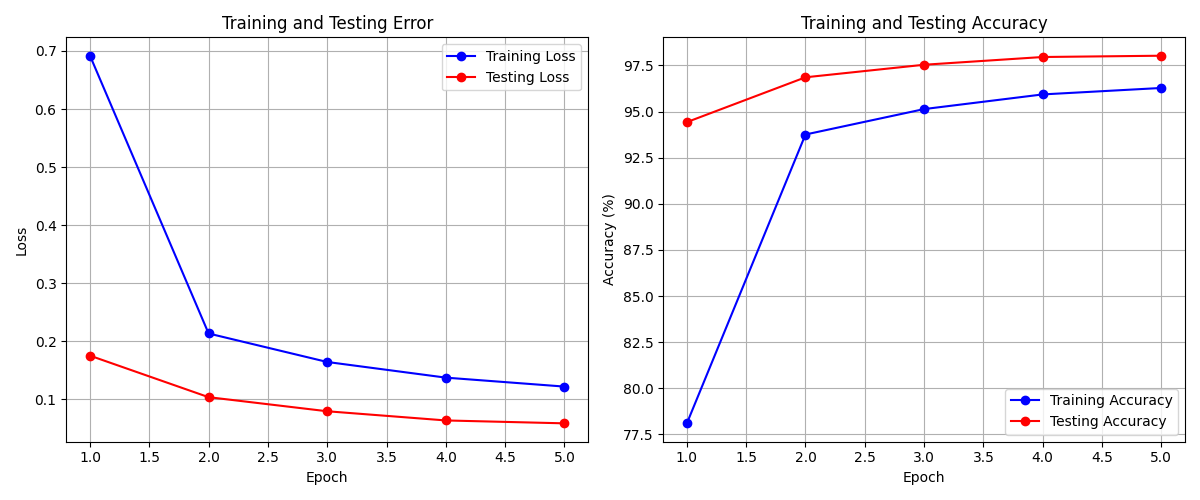
\includegraphics[width=\textwidth]{plot_training_results.png}
    \caption{Training and testing loss (left) and accuracy (right) over 5 epochs. Blue represents training, red represents testing. Both loss and accuracy converge steadily.}
    \label{fig:training}
\end{figure}

\subsection{D -- Saving the Network}

The trained model weights were saved to \texttt{mnist\_model.pth} using \texttt{torch.save(model.state\_dict(), ...)}.

\subsection{E -- Testing on the Test Set}

The saved model was loaded in a separate file (\texttt{test\_mnist.py}) and evaluated on the first 10 test examples. The network was set to evaluation mode (\texttt{model.eval()}) to disable dropout. Table~\ref{tab:first10} shows the network outputs for the first 10 test examples.

\begin{table}[H]
\centering
\caption{Network output values for the first 10 test examples (log probabilities). The predicted class matches the true label for all 10 examples.}
\label{tab:first10}
\small
\begin{tabular}{@{}ccc@{}}
\toprule
\textbf{Index} & \textbf{Predicted} & \textbf{True Label} \\
\midrule
0 & 7 & 7 \\
1 & 2 & 2 \\
2 & 1 & 1 \\
3 & 0 & 0 \\
4 & 4 & 4 \\
5 & 1 & 1 \\
6 & 4 & 4 \\
7 & 9 & 9 \\
8 & 5 & 5 \\
9 & 9 & 9 \\
\bottomrule
\end{tabular}
\end{table}

Figure~\ref{fig:predictions} shows the first 9 test digits in a 3$\times$3 grid with their predictions.

\begin{figure}[H]
    \centering
    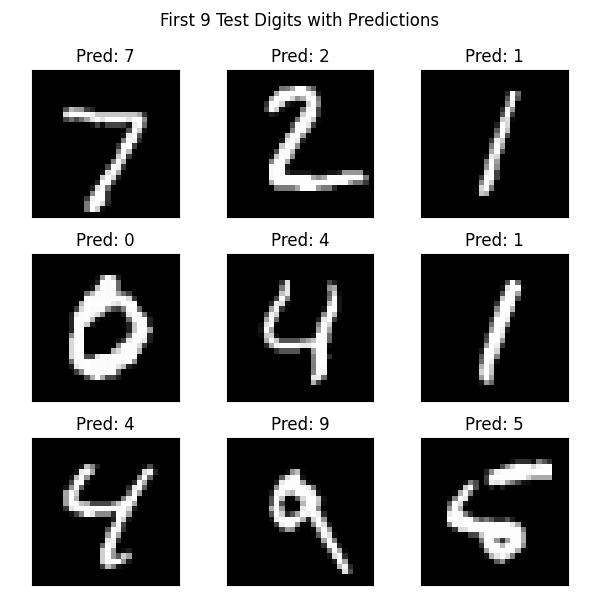
\includegraphics[width=0.55\textwidth]{plot_predictions.png}
    \caption{First 9 test digits with model predictions shown above each image. All predictions are correct.}
    \label{fig:predictions}
\end{figure}

\subsection{F -- Testing on Custom Handwritten Digits}

I wrote digits 0--9 on white paper with a thick marker, photographed them, cropped each digit individually, and ran them through the network. The images were converted to grayscale, inverted (to match MNIST's white-on-black format), and resized to 28$\times$28. Figure~\ref{fig:custom_digits} shows the results. The network correctly classified 8 out of 10 custom digits, misclassifying digits 3 and 6.

\begin{figure}[H]
    \centering
    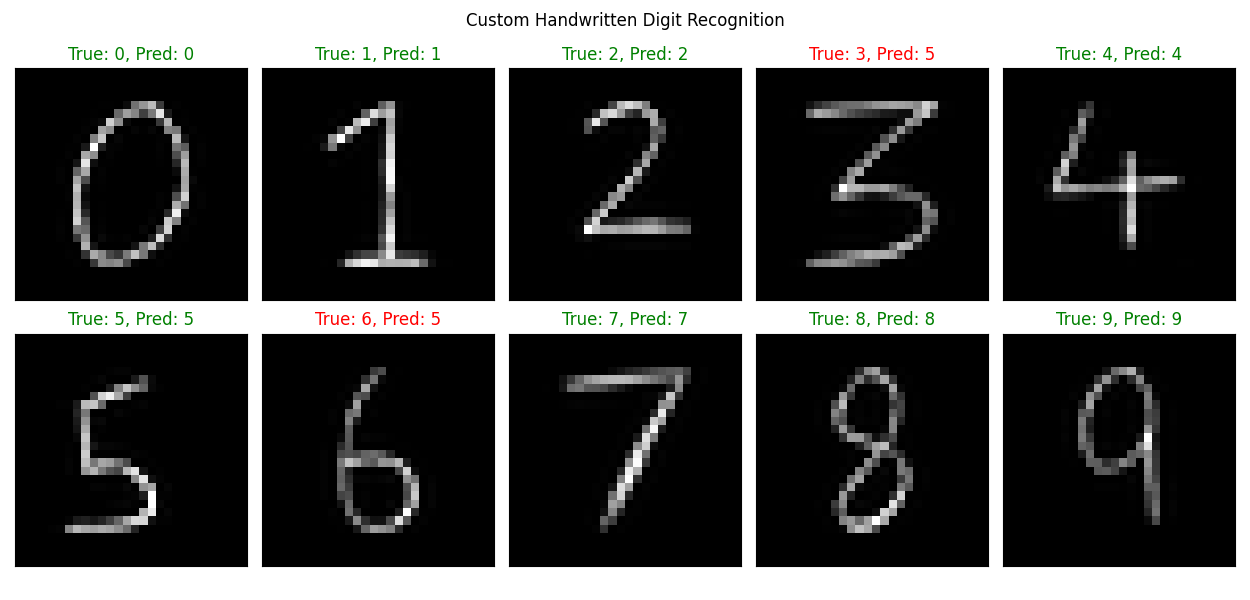
\includegraphics[width=\textwidth]{plot_custom_digits.png}
    \caption{Custom handwritten digit recognition results. Green titles indicate correct predictions; red indicates misclassifications. The network misclassified 3 as 5 and 6 as 5.}
    \label{fig:custom_digits}
\end{figure}

\newpage
% ============================================================
\section{Task 2: Examine Your Network}
% ============================================================

\subsection{A -- Analyzing the First Layer}

The first convolutional layer (\texttt{conv1}) contains 10 filters of size 5$\times$5 with 1 input channel. The filter weight tensor has shape [10, 1, 5, 5]. Figure~\ref{fig:conv1_filters} shows the 10 learned filters visualized as grayscale images.

\begin{figure}[H]
    \centering
    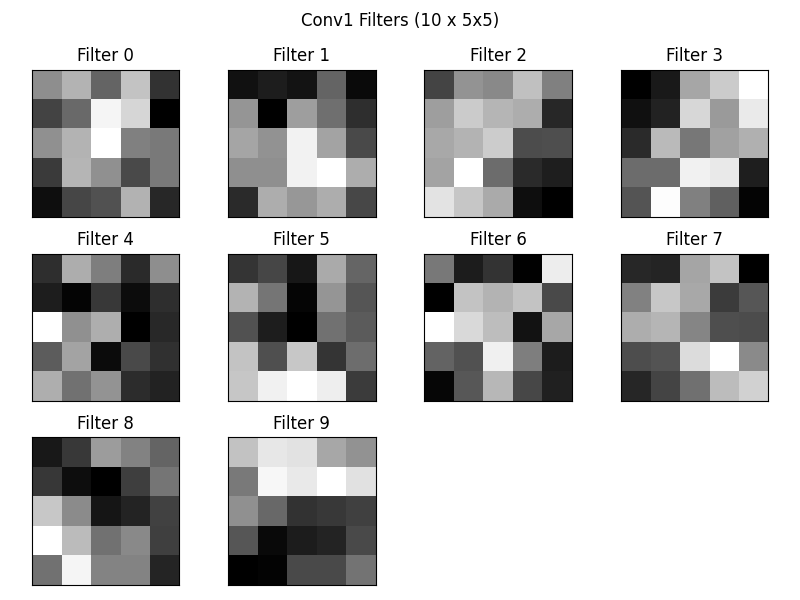
\includegraphics[width=0.65\textwidth]{conv1_filters.png}
    \caption{Visualization of the 10 learned conv1 filters (5$\times$5). Each filter detects different edge orientations and patterns. Lighter pixels represent larger positive weights; darker pixels represent negative weights.}
    \label{fig:conv1_filters}
\end{figure}

\subsection{B -- Effect of the Filters}

Each of the 10 filters was applied to the first training image (digit 5) using OpenCV's \texttt{filter2D} function. Figure~\ref{fig:conv1_results} shows the filter and its effect side by side.

\begin{figure}[H]
    \centering
    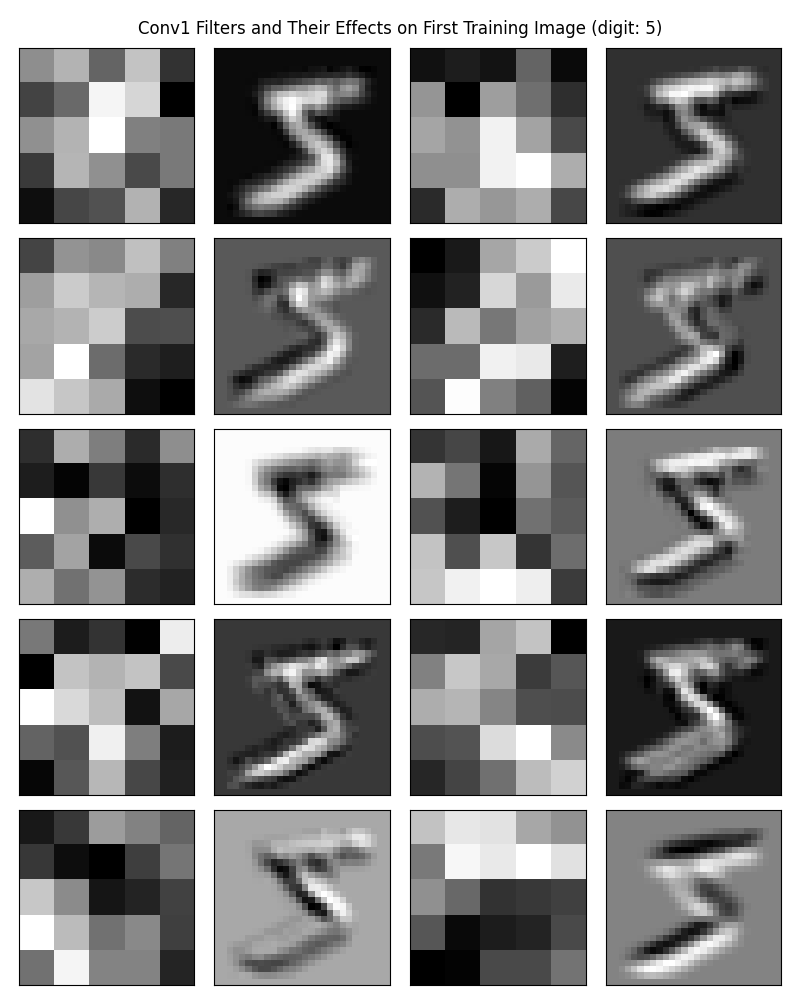
\includegraphics[width=0.65\textwidth]{conv1_filterResults.png}
    \caption{Conv1 filters (columns 1, 3) and their filtered output (columns 2, 4) applied to the first training image (digit 5). Different filters highlight different edges and features of the digit.}
    \label{fig:conv1_results}
\end{figure}

The results make sense given the filters. Filters with strong horizontal gradients (light on top, dark on bottom or vice versa) highlight horizontal edges of the digit, while filters with vertical gradients emphasize vertical strokes. Some filters act as edge detectors at specific orientations, producing bright responses where the digit's contour aligns with that orientation.

\newpage
% ============================================================
\section{Task 3: Transfer Learning on Greek Letters}
% ============================================================

To recognize Greek letters (alpha, beta, gamma), I adapted the pre-trained MNIST CNN by:
\begin{enumerate}[nosep]
    \item Loading the trained MNIST model weights
    \item Freezing all network parameters (\texttt{param.requires\_grad = False})
    \item Replacing the final fully connected layer (\texttt{fc2}) from 10 outputs to 3 outputs
\end{enumerate}

The modified network structure:
\begin{verbatim}
MyNetwork(
  (conv1): Conv2d(1, 10, kernel_size=(5, 5))    [frozen]
  (conv2): Conv2d(10, 20, kernel_size=(5, 5))   [frozen]
  (conv2_drop): Dropout2d(p=0.5)                [frozen]
  (fc1): Linear(in=320, out=50)                 [frozen]
  (fc2): Linear(in=50, out=3)                   [trainable]
)
\end{verbatim}

The 27 Greek letter training images (133$\times$133, RGB) were transformed to match MNIST format using grayscale conversion, scaling, center cropping to 28$\times$28, and intensity inversion. Training used SGD with learning rate 0.01 and batch size 5.

Figure~\ref{fig:greek_training} shows the training loss over epochs. The network reached near-perfect accuracy on the 27 training examples within approximately 25 epochs.

\begin{figure}[H]
    \centering
    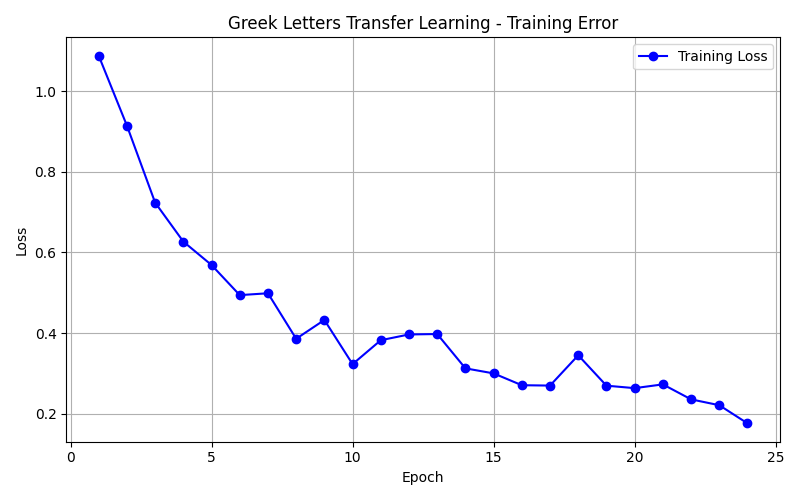
\includegraphics[width=0.7\textwidth]{greek_training_error.png}
    \caption{Training loss for Greek letter transfer learning. Loss decreases steadily from 1.1 to below 0.2 over 25 epochs.}
    \label{fig:greek_training}
\end{figure}

I also tested the network on my own handwritten Greek letters. Figure~\ref{fig:greek_custom} shows the results. The network correctly classified most custom examples, with some misclassifications on alpha symbols that were written with different style variations.

\begin{figure}[H]
    \centering
    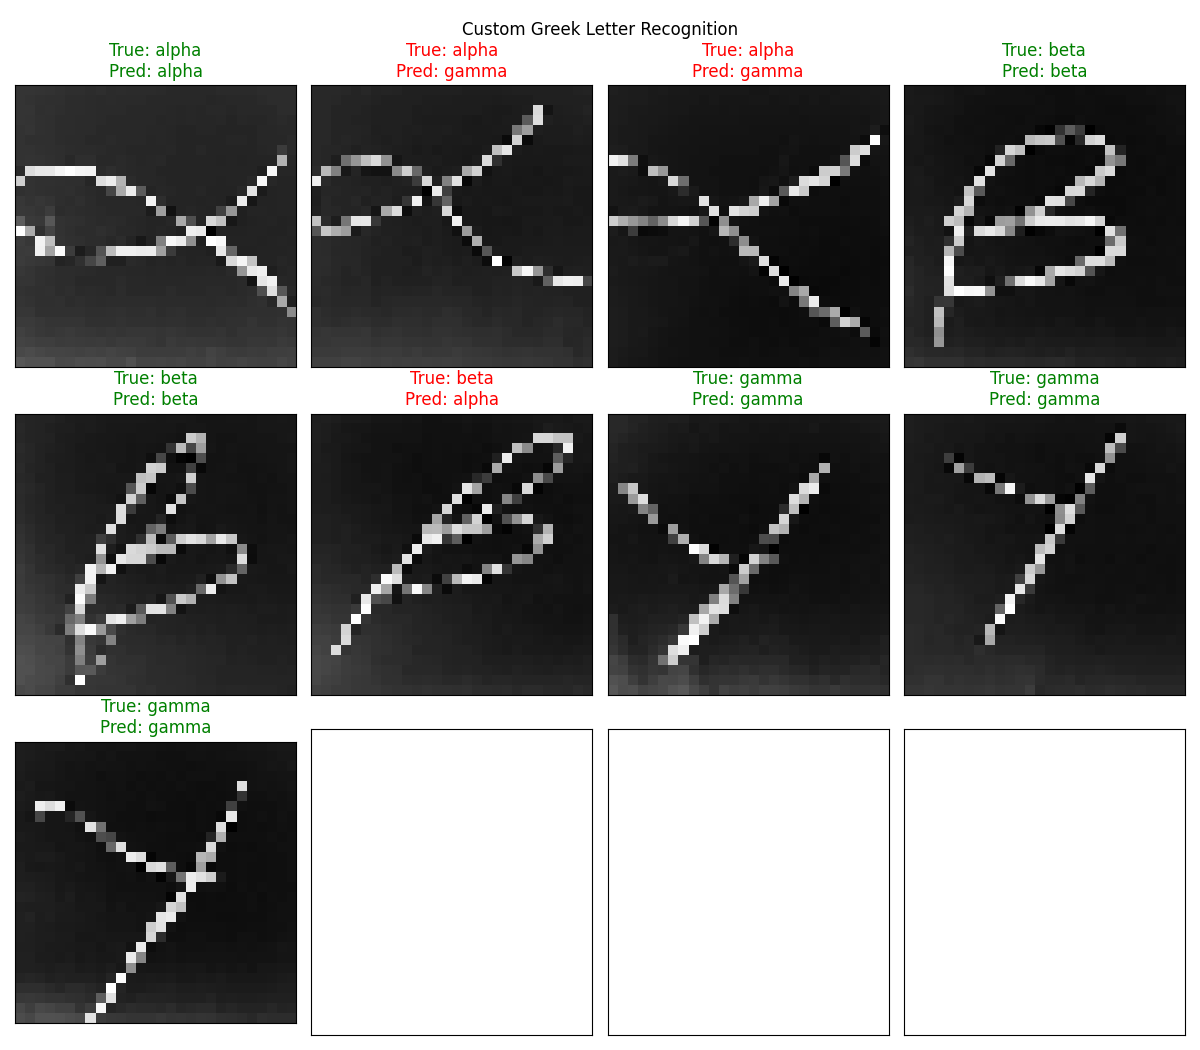
\includegraphics[width=0.85\textwidth]{greek_custom_results.png}
    \caption{Custom Greek letter recognition results. Green indicates correct predictions; red indicates misclassifications. The network struggled with some alpha variations.}
    \label{fig:greek_custom}
\end{figure}

\newpage
% ============================================================
\section{Task 4: Transformer Network}
% ============================================================

I re-implemented the MNIST recognition network using a Vision Transformer (ViT) architecture. The key components are:

\begin{enumerate}[nosep]
    \item \textbf{Patch Embedding}: Images are divided into overlapping patches (size 4, stride 2) using \texttt{nn.Unfold}, producing 169 tokens. Each patch is projected to a 48-dimensional embedding via a linear layer.
    \item \textbf{Positional Embedding}: Learnable positional embeddings are added to each token.
    \item \textbf{Transformer Encoder}: 4 transformer encoder layers with 8 attention heads, feedforward dimension 128, GELU activation, and pre-norm architecture.
    \item \textbf{Classification}: Token outputs are averaged (global average pooling), passed through LayerNorm, then a two-layer MLP (48 $\rightarrow$ 128 $\rightarrow$ 10) with GELU activation and log-softmax output.
\end{enumerate}

The transformer was trained using AdamW optimizer with learning rate $10^{-3}$ and weight decay $10^{-4}$ for 5 epochs. Figure~\ref{fig:transformer_training} shows the training results. The transformer achieved approximately 97\% test accuracy, comparable to the CNN.

\begin{figure}[H]
    \centering
    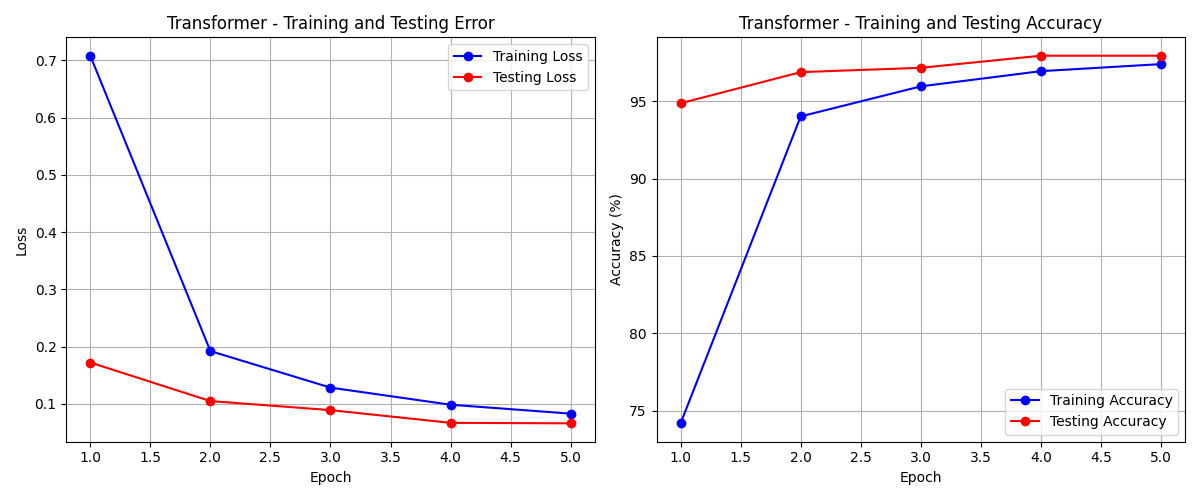
\includegraphics[width=\textwidth]{transformer_training_results.png}
    \caption{Transformer training and testing loss (left) and accuracy (right) over 5 epochs on MNIST. The model reaches 97\% test accuracy, comparable to the CNN.}
    \label{fig:transformer_training}
\end{figure}

\newpage
% ============================================================
\section{Task 5: Experiment -- Transformer Architecture Search}
% ============================================================

\subsection{A -- Plan}

I evaluated the Vision Transformer on the \textbf{Fashion MNIST} dataset (more challenging than digits) along three dimensions:

\begin{itemize}[nosep]
    \item \textbf{Dimension 1 -- Depth} (number of transformer layers): [1, 2, 3, 4]
    \item \textbf{Dimension 2 -- Attention Heads}: [1, 2, 4, 8]
    \item \textbf{Dimension 3 -- Dropout Rate}: [0.0, 0.1, 0.2, 0.5]
\end{itemize}

I used a \textbf{round-robin linear search} strategy: hold two dimensions constant, sweep the third, select the best value, then move to the next dimension. This was repeated for 2 rounds, totaling \textbf{24 runs} (automated). Each run trained for 2 epochs with batch size 128 on a GPU (NVIDIA GTX 1650). The metric used was test set accuracy.

\subsection{B -- Hypotheses}

\begin{itemize}[nosep]
    \item \textbf{H1 (Depth)}: Increasing depth will improve accuracy up to 3--4 layers, then plateau or decrease due to overfitting.
    \item \textbf{H2 (Heads)}: More attention heads should help up to 4--6, but too many with embed\_dim=48 will hurt because each head gets very few dimensions.
    \item \textbf{H3 (Dropout)}: A small dropout (0.1--0.2) should improve generalization. Too much ($>$0.3) will hurt accuracy.
\end{itemize}

\subsection{C -- Results}

Figure~\ref{fig:experiment_summary} shows the results across all three dimensions over both rounds.

\begin{figure}[H]
    \centering
    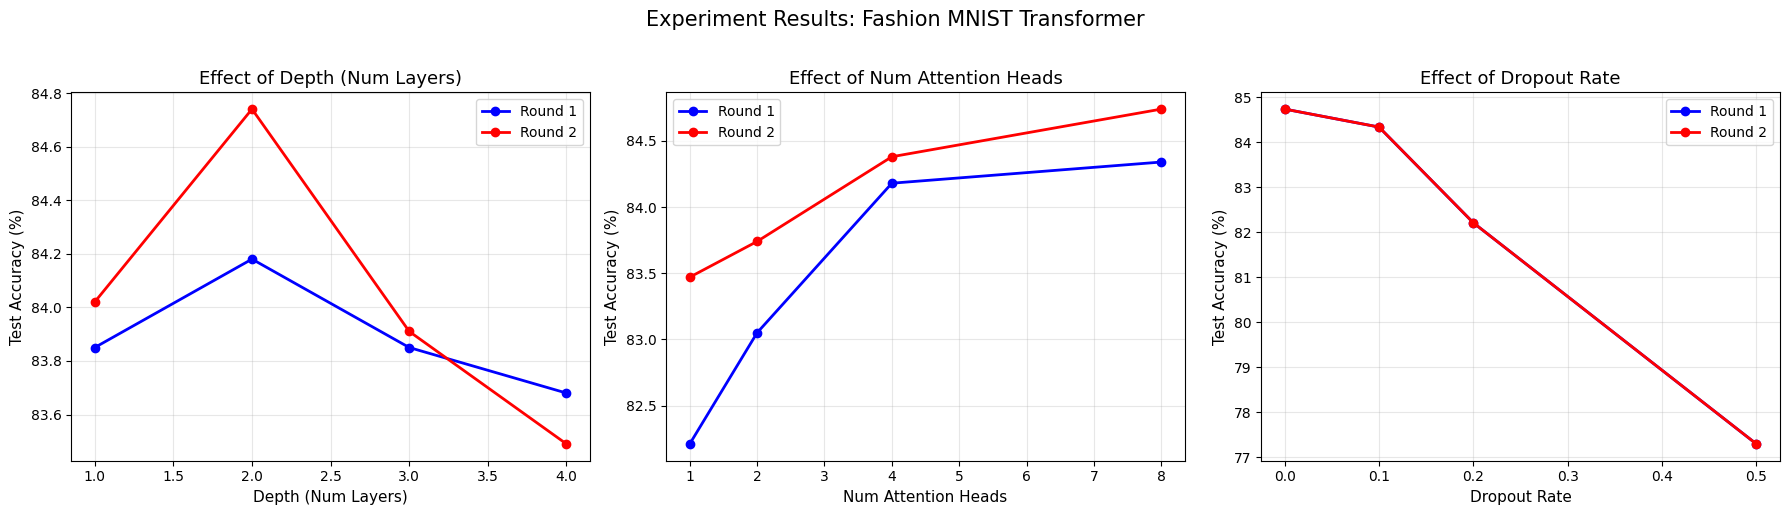
\includegraphics[width=\textwidth]{experiment_summary.png}
    \caption{Experiment results for Fashion MNIST transformer. Left: effect of depth. Center: effect of attention heads. Right: effect of dropout rate. Blue = Round 1, Red = Round 2.}
    \label{fig:experiment_summary}
\end{figure}

\begin{table}[H]
\centering
\caption{Optimized transformer parameters for Fashion MNIST}
\label{tab:experiment_results}
\begin{tabular}{@{}lccc@{}}
\toprule
\textbf{Dimension} & \textbf{Best Value} & \textbf{Test Accuracy} & \textbf{Hypothesis} \\
\midrule
Depth (Num Layers) & 2 & 84.74\% & Supported \\
Attention Heads & 8 & 84.74\% & Partially Supported \\
Dropout Rate & 0.0 & 84.74\% & Rejected \\
\bottomrule
\end{tabular}
\end{table}

\textbf{Analysis of Hypotheses:}
\begin{itemize}[nosep]
    \item \textbf{H1 (Depth) -- Supported}: Accuracy peaked at depth=2 (84.74\%) and decreased with more layers. With only 2 training epochs, deeper models could not converge, confirming that more layers can hurt when training time is limited.
    \item \textbf{H2 (Heads) -- Partially Supported}: More heads consistently improved accuracy (1$\rightarrow$8 monotonically). Contrary to the hypothesis, 8 heads performed best even with embed\_dim=48 (6 dimensions per head), suggesting the model benefits from more diverse attention patterns.
    \item \textbf{H3 (Dropout) -- Rejected}: Zero dropout gave the best results. With only 2 epochs of training, the model had not yet overfit, so dropout only removed useful information during training without providing regularization benefits.
\end{itemize}

The total experiment ran 24 configurations in 33.7 minutes on a NVIDIA GeForce GTX 1650 GPU.

\newpage
% ============================================================
\section{Extensions}
% ============================================================

\subsection{Extension 1: Pre-trained VGG16 Network Analysis}

I loaded a pre-trained VGG16 network (trained on ImageNet) and visualized its first two convolutional layers, similar to the analysis in Task 2. VGG16's first layer has 64 RGB 3$\times$3 filters, compared to the MNIST CNN's 10 grayscale 5$\times$5 filters.

\begin{figure}[H]
    \centering
    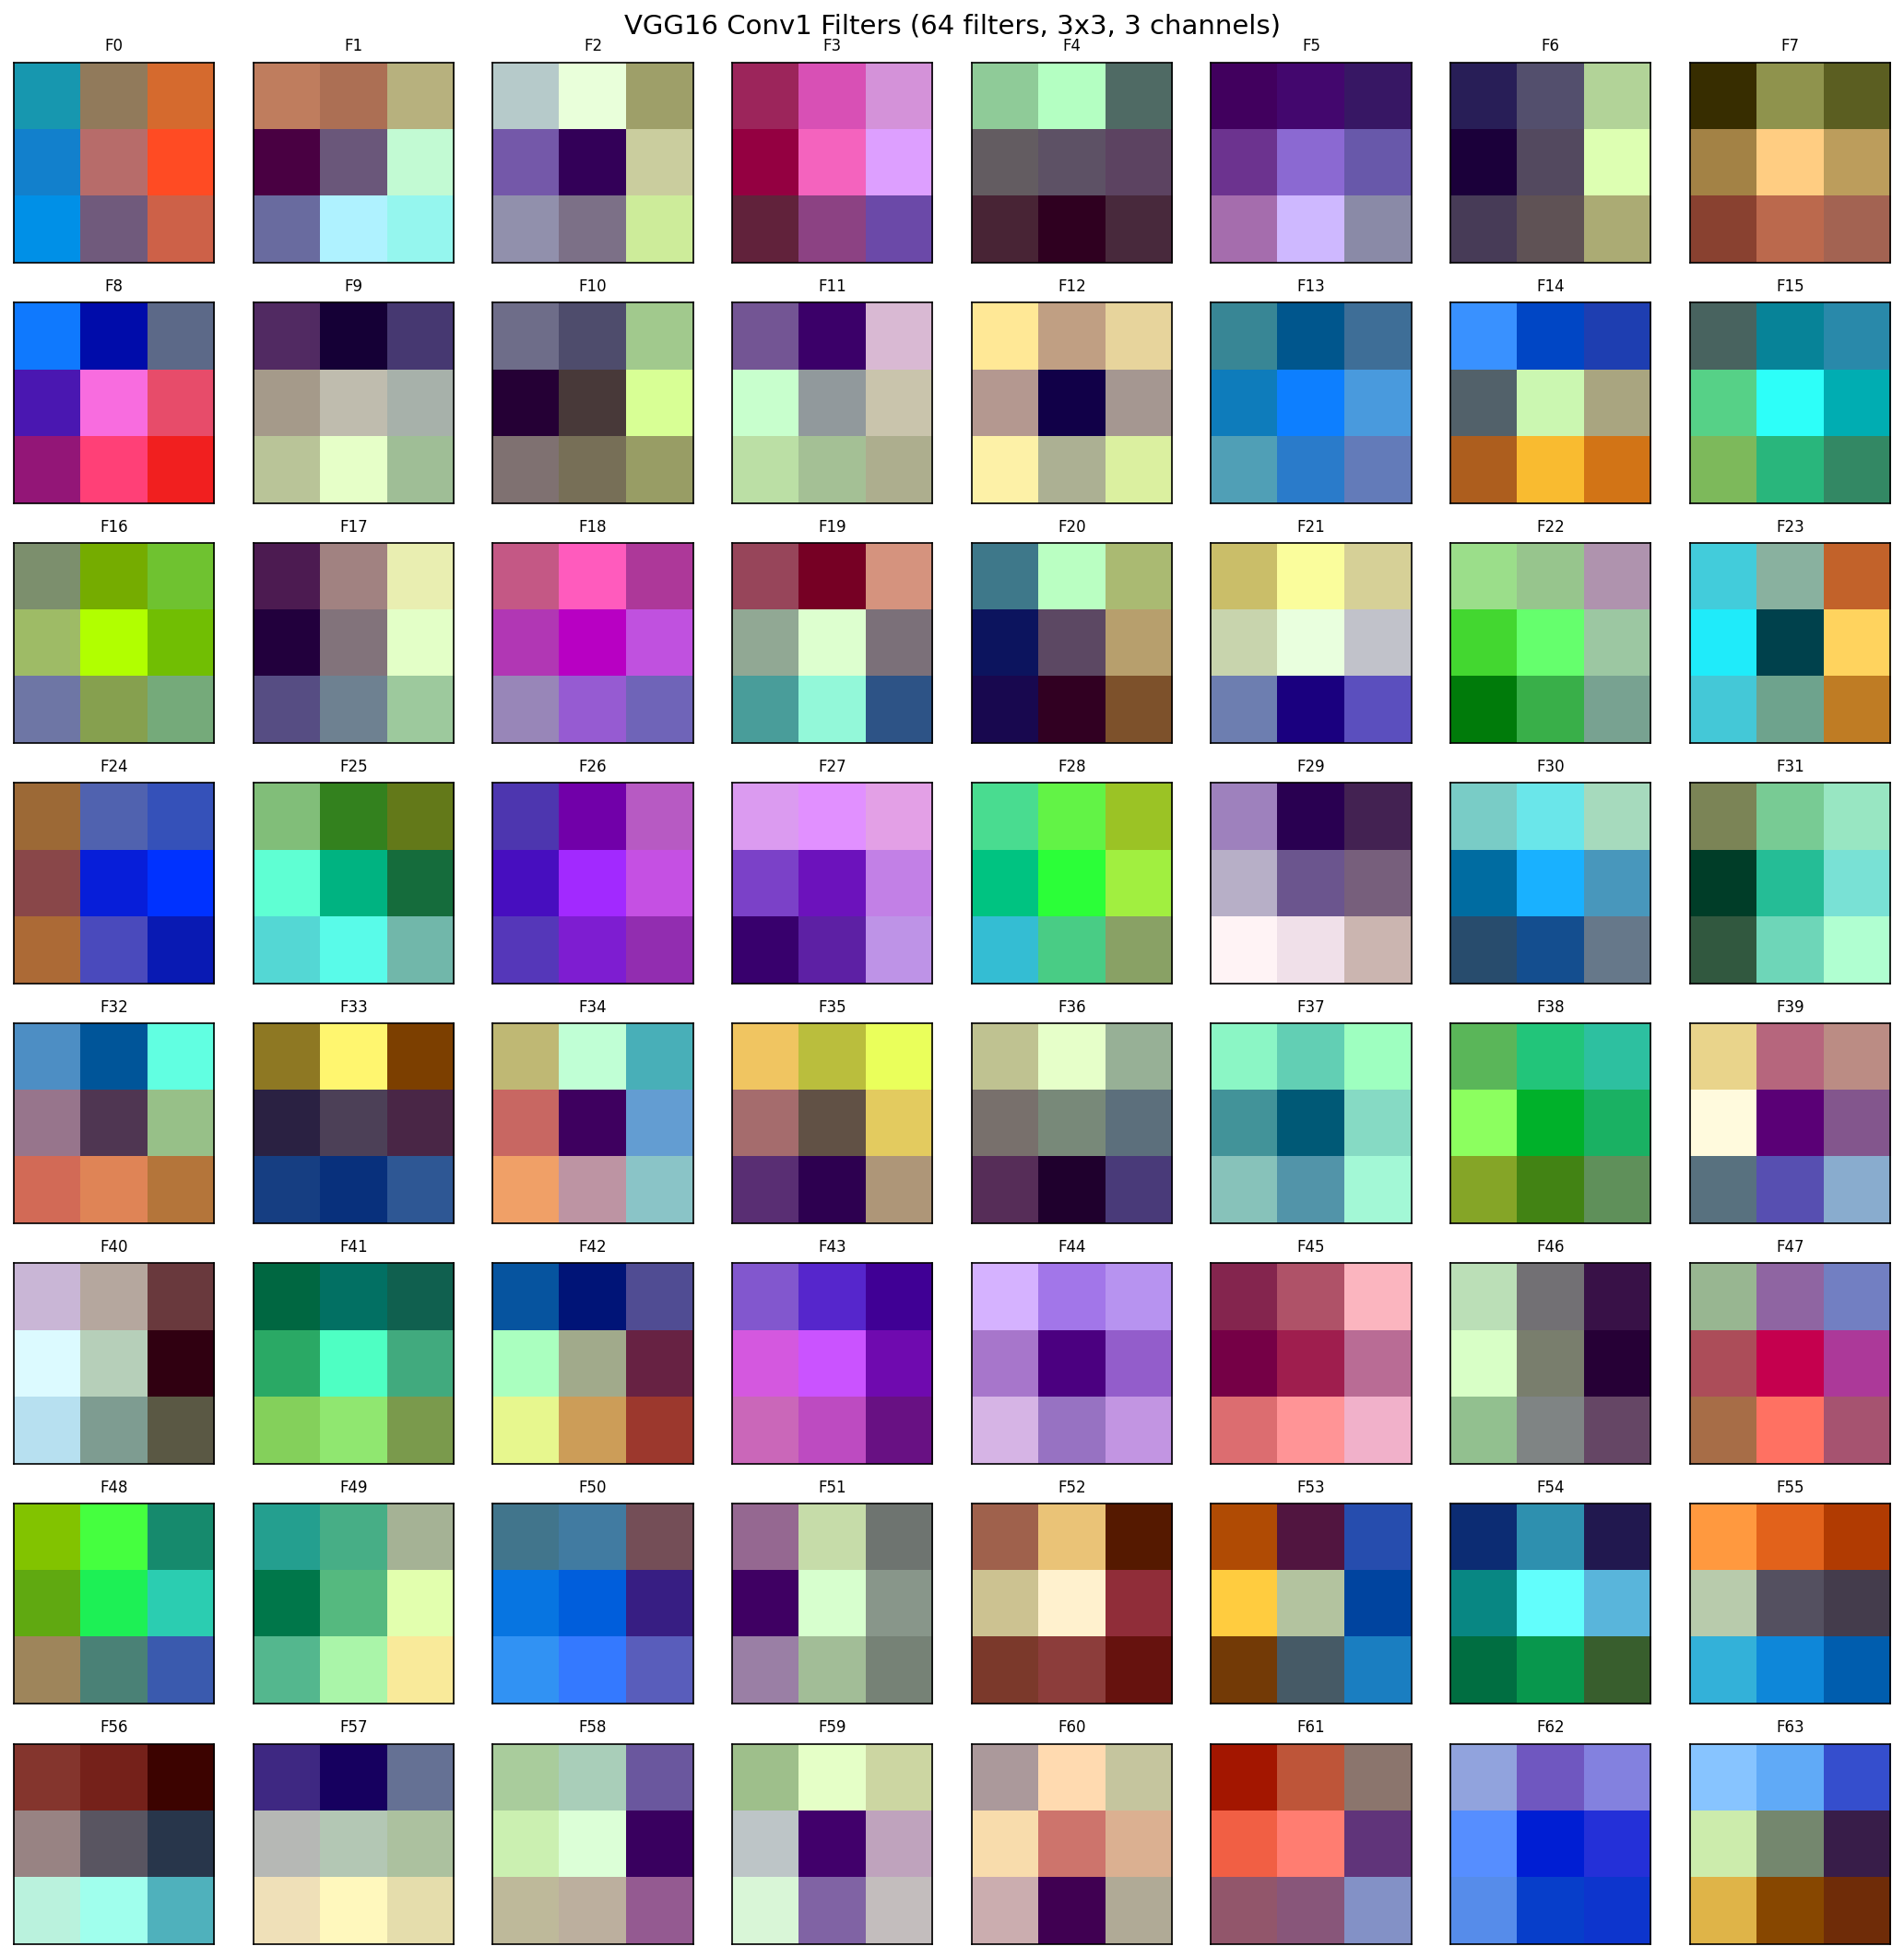
\includegraphics[width=0.85\textwidth]{ext_vgg16_conv1_filters.png}
    \caption{VGG16 Conv1 filters (64 filters, 3$\times$3, 3 channels displayed as RGB). These filters detect various color gradients and edge orientations.}
    \label{fig:vgg_conv1}
\end{figure}

\begin{figure}[H]
    \centering
    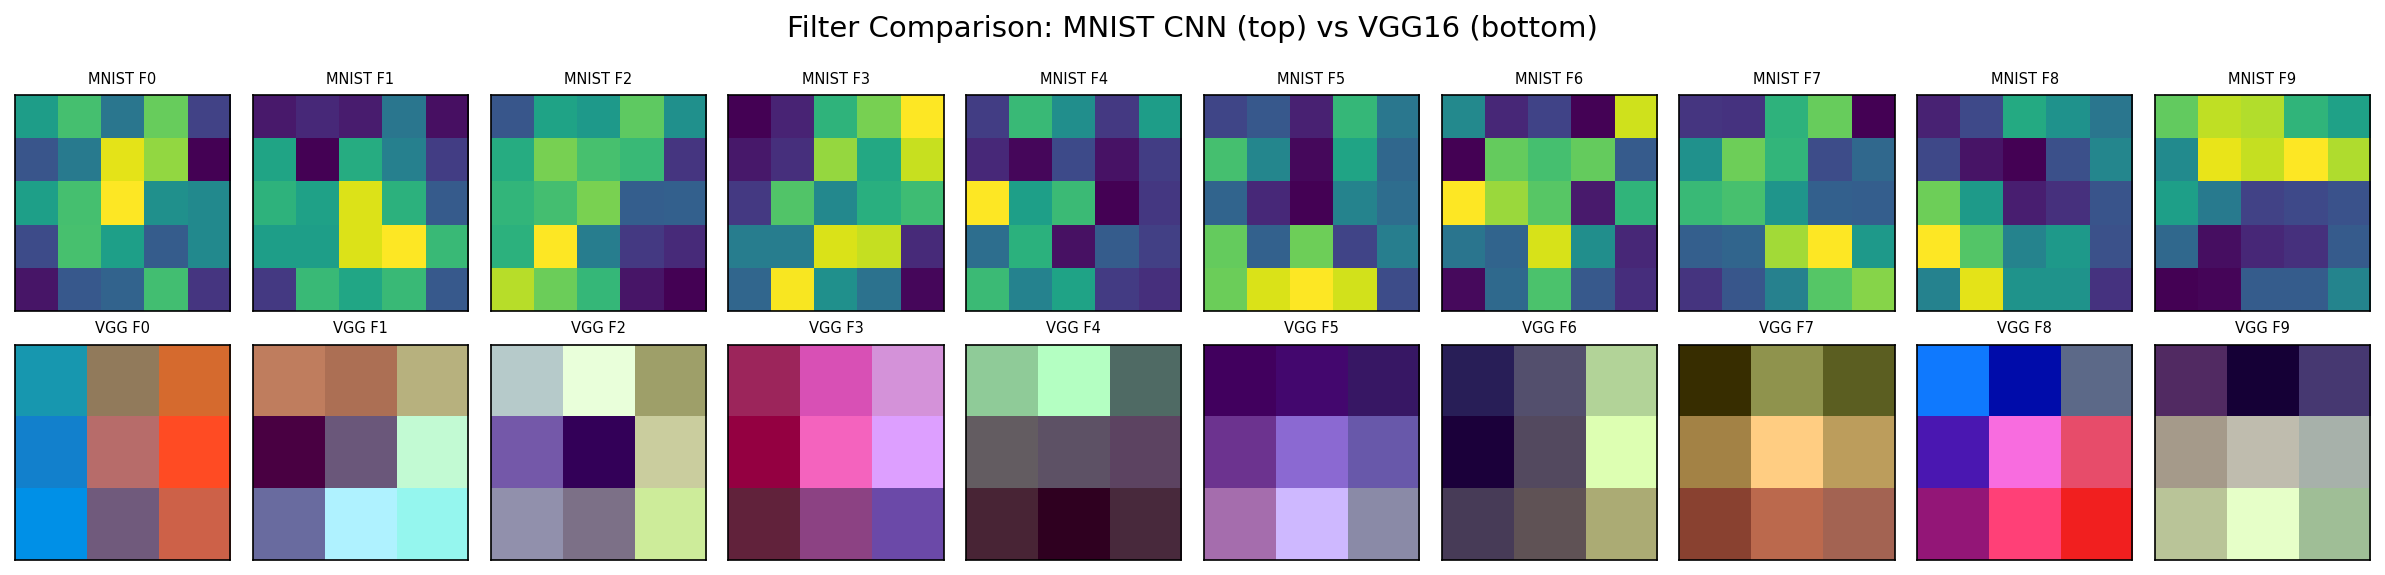
\includegraphics[width=\textwidth]{ext_filter_comparison.png}
    \caption{Comparison of MNIST CNN filters (top row, 5$\times$5 grayscale) vs VGG16 filters (bottom row, 3$\times$3 RGB). VGG16 filters show more color variety since they were trained on natural images.}
    \label{fig:filter_comparison}
\end{figure}

I also applied VGG16's 64 conv1 filters to an MNIST digit image. Figure~\ref{fig:vgg_results} shows that even though VGG16 was trained on natural color images, its edge-detection filters still produce meaningful feature maps when applied to grayscale digit images.

\begin{figure}[H]
    \centering
    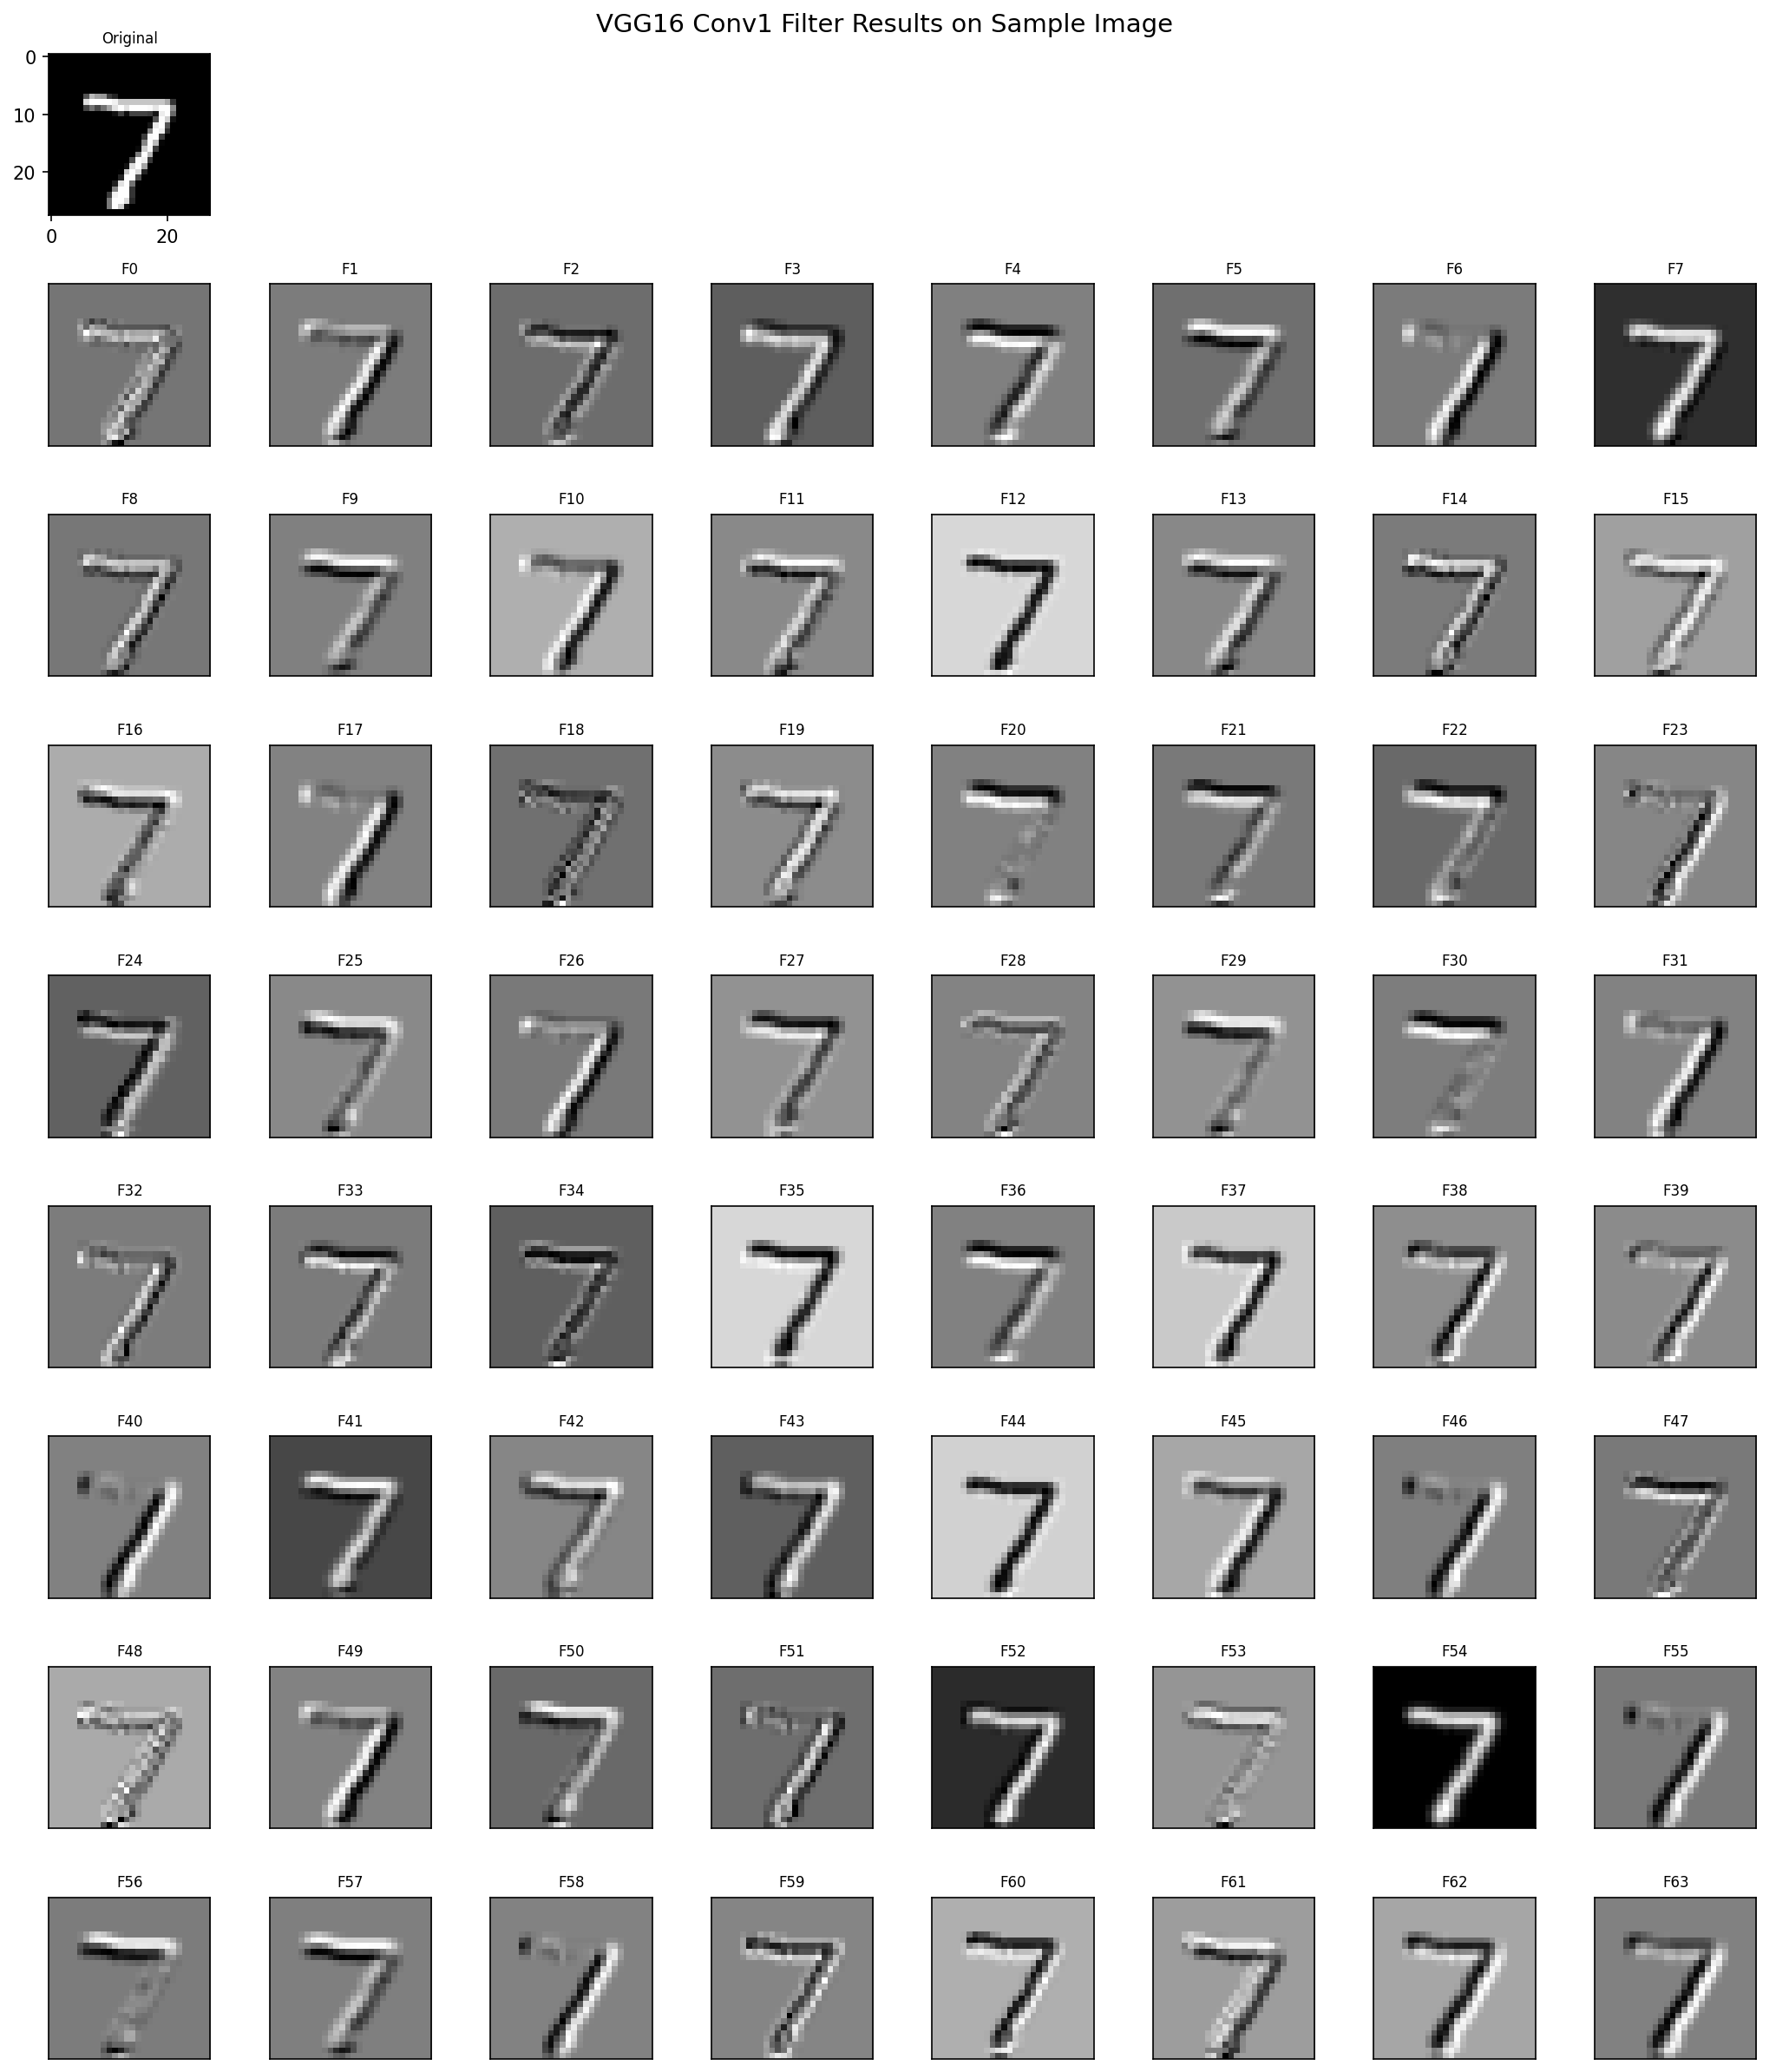
\includegraphics[width=0.6\textwidth]{ext_vgg16_conv1_results.png}
    \caption{VGG16 Conv1 filter results applied to MNIST digit 7. Despite being trained on natural images, the filters highlight edges and contours of the digit effectively.}
    \label{fig:vgg_results}
\end{figure}

\subsection{Extension 2: Live Video Digit Recognition}

I built a real-time digit recognition application using the trained MNIST CNN and OpenCV's webcam capture. The application:
\begin{itemize}[nosep]
    \item Opens the webcam and displays a green bounding box for the region of interest
    \item Preprocesses each frame: converts to grayscale, applies Otsu thresholding, inverts colors, and resizes to 28$\times$28
    \item Runs the preprocessed image through the CNN and displays the prediction with confidence
    \item Shows a probability bar chart for all 10 classes and a preview of what the model sees
\end{itemize}

A video demonstration of the live recognition system is available here: \url{https://drive.google.com/file/d/1iI77E1l0X-Fd401YFDDWgRRz_0TpC-K3/view?usp=sharing}. The system runs at real-time frame rates and successfully recognizes digits held up to the camera when written with thick dark strokes on white paper.

\newpage
% ============================================================
\section{Reflection}
% ============================================================

This project taught me several key lessons about deep learning:
\begin{itemize}[nosep]
    \item \textbf{CNN fundamentals}: Understanding how convolutional filters learn to detect features at different levels of abstraction, from edges in early layers to more complex patterns in deeper layers.
    \item \textbf{Transfer learning}: Freezing pre-trained weights and fine-tuning only the final layer is remarkably effective even with very few examples (27 Greek letter images).
    \item \textbf{Transformers for vision}: Vision Transformers can match CNN performance on simple tasks like MNIST, but require careful tuning of patch size, embedding dimension, and depth.
    \item \textbf{Hyperparameter sensitivity}: The Task 5 experiment showed that dropout can actually hurt when training is short, and that more is not always better for network depth.
    \item \textbf{GPU utilization}: Understanding how to properly move models and data to GPU, and that small models may not fully utilize GPU capacity.
\end{itemize}

% ============================================================
\section{Acknowledgements}
% ============================================================

\begin{itemize}[nosep]
    \item PyTorch documentation and tutorials (\url{https://pytorch.org/tutorials/})
    \item PyTorch MNIST example: \url{https://github.com/pytorch/examples/tree/main/mnist}
    \item MNIST dataset by Yann LeCun, Corinna Cortes, and Christopher J.C. Burges (\url{http://yann.lecun.com/exdb/mnist/})
    \item Fashion MNIST dataset by Zalando Research (\url{https://github.com/zalandoresearch/fashion-mnist})
    \item VGG16 pre-trained weights from torchvision model zoo, originally trained on ImageNet (Simonyan \& Zisserman, 2014)
    \item ``An Image is Worth 16x16 Words: Transformers for Image Recognition at Scale'' -- Dosovitskiy et al., 2020 (\url{https://arxiv.org/abs/2010.11929})
    \item OpenCV documentation for image processing and webcam capture (\url{https://docs.opencv.org/})
    \item Course lectures and office hours with the instructor
\end{itemize}

\end{document}
